% ================================================================
\section{Methodology}
% ================================================================

\subsection{Pipeline Overview}

The Completus pipeline consists of five sequential stages: (1) data
collection and preprocessing, (2) QLoRA fine-tuning, (3) adapter
merging, (4) GGUF export and quantisation, and (5) Ollama
registration. Fig.~\ref{fig:pipeline} illustrates the complete
end-to-end flow.

\begin{figure}[htbp]
  \centering
  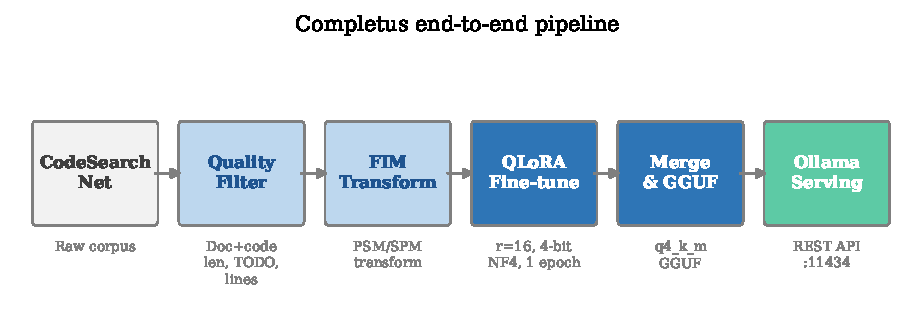
\includegraphics[width=\textwidth]{fig_pipeline.pdf}
  \caption{Completus end-to-end pipeline. Raw CodeSearchNet samples
  pass through quality filtering and a fill-in-the-middle transform,
  are used to fine-tune Qwen2.5-Coder-1.5B via QLoRA, and the merged
  adapter is exported to GGUF q4\_k\_m and served locally through
  Ollama.}
  \label{fig:pipeline}
\end{figure}

\subsection{Dataset and Preprocessing}

We use CodeSearchNet~\cite{Husain2019CSN}
(\texttt{claudios/code\_search\_net} on HuggingFace Hub), a corpus of
paired function and docstring tuples extracted from open-source
repositories. The full training splits contain 412,178 Python and
317,832 Go functions. To keep preparation tractable on a single
workstation, we cap the pipeline input at the first 50,000 functions
per language and process them through five sequential stages:
\begin{enumerate}[leftmargin=16pt]
  \item \textit{Near-deduplication}: MinHash LSH with 128 permutations,
        5-token shingles, and a Jaccard threshold of 0.8.
  \item \textit{Code-smell filtering}: drop functions with any line
        exceeding 120 characters, fewer than 30 tokens, or a no-op
        body (bare \texttt{pass}, ellipsis, or empty return);
        normalise indentation on the rest.
  \item \textit{Docstring filtering}: require at least 15 tokens, at
        least two words, no \texttt{TODO}/\texttt{FIXME}/\texttt{XXX}
        markers, and a docstring distinct from the function name.
  \item \textit{Fill-in-the-middle transform} (described below).
  \item \textit{Length management}: enforce the 2048-token limit.
\end{enumerate}
Table~\ref{tab:dataset} reports counts before and after the pipeline;
Fig.~\ref{fig:dataset} visualises the result.

\begin{table}[htbp]
  \centering
  \caption{Training Data After the Preparation Pipeline}
  \label{tab:dataset}
  \begin{tabular}{lrrr}
    \toprule
    \textbf{Language} & \textbf{Input cap} & \textbf{After pipeline} & \textbf{Retained} \\
    \midrule
    Python & 50{,}000 & 31{,}966 & 63.9\% \\
    Go     & 50{,}000 & 21{,}284 & 42.6\% \\
    \midrule
    Total  & 100{,}000 & 53{,}250 & 53.3\% \\
    \bottomrule
  \end{tabular}
\end{table}

\begin{figure}[htbp]
  \centering
  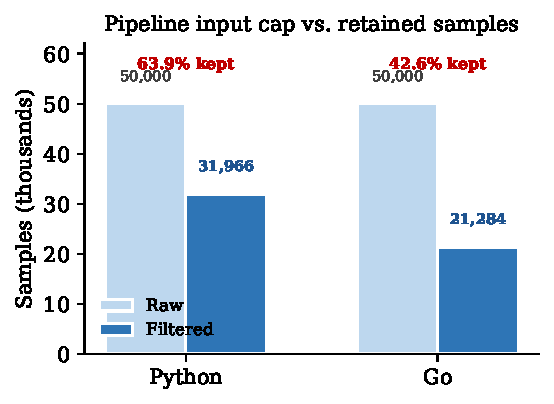
\includegraphics[width=0.6\textwidth]{fig_dataset.pdf}
  \caption{Training samples retained from the 50,000-function input cap
  per language after the five-stage preparation pipeline: 31,966
  Python (63.9\%) and 21,284 Go (42.6\%).}
  \label{fig:dataset}
\end{figure}

For the fill-in-the-middle stage we follow Bavarian et
al.~\cite{Bavarian2022FIM}: 80\% of samples receive the transform,
in which a span of the function body is extracted, moved to the end
of the sequence, and delimited with the model's
\texttt{<|fim\_prefix|>}, \texttt{<|fim\_suffix|>}, and
\texttt{<|fim\_middle|>} sentinel tokens. The remaining 20\% are kept
as plain left-to-right samples.

\subsection{Model and QLoRA Fine-Tuning}

We fine-tune Qwen2.5-Coder-1.5B~\cite{Hui2024Qwen25} loaded in 4-bit
NF4 quantisation using the QLoRA protocol~\cite{Dettmers2023QLoRA}
via Unsloth. LoRA adapters are attached to all seven linear projection
matrices (q, k, v, o, gate, up, down) with rank $r=16$ and scaling
factor $\alpha=32$. Table~\ref{tab:hyperparams} lists all
hyperparameters.

\begin{table}[htbp]
  \centering
  \caption{QLoRA Fine-Tuning Hyperparameters}
  \label{tab:hyperparams}
  \begin{tabular}{ll}
    \toprule
    \textbf{Hyperparameter} & \textbf{Value} \\
    \midrule
    Base model       & Qwen2.5-Coder-1.5B \\
    Quantisation     & 4-bit NF4 (QLoRA) \\
    LoRA rank $r$    & 16 \\
    LoRA $\alpha$    & 32 \\
    Target modules   & q, k, v, o, gate, up, down \\
    Batch size       & 2 (per device) \\
    Gradient accum.  & 8 (effective batch 16) \\
    Learning rate    & $2 \times 10^{-4}$ \\
    LR scheduler     & Cosine \\
    Warmup steps     & 10 \\
    Optimiser        & AdamW 8-bit \\
    Epochs           & 1 \\
    Max seq.\ length & 2048 \\
    Seed             & 3407 \\
    Hardware         & NVIDIA RTX 4060 Laptop (8\,GB) \\
    \bottomrule
  \end{tabular}
\end{table}

Each language is trained for one epoch: 1,998 gradient steps for
Python (31,966 samples) and 1,331 for Go (21,284 samples) at an
effective batch size of 16. The Go run completed in 3,713 seconds
(62 minutes); the Python run, at a slower per-step rate due to longer
average sequences, took approximately 2.2 hours. The initial training
loss for the Python run was 1.674, and the Go run reached a final mean
training loss of 1.111 under the cosine schedule.

\subsection{Adapter Merging and GGUF Export}

After training, the LoRA adapter weights are merged into the base
model using Unsloth's GGUF export routine, which simultaneously
writes the merged safetensors checkpoint and a quantised GGUF binary.
We select the q4\_k\_m quantisation scheme, characterised by
Kurt~\cite{Kurt2026Quant} as achieving a favourable
perplexity-size trade-off at this scale.

\subsection{Local Serving with Ollama}

Each GGUF binary is registered with Ollama using a Modelfile that
specifies the FIM prompt template and generation parameters:
temperature 0.0 for deterministic completions, \texttt{num\_ctx} 2048,
and \texttt{num\_predict} 256 tokens. The registered models are
queryable at \texttt{http://localhost:11434} through Ollama's local
REST API.
